\section{Mehrdimensionale Wahrscheinlichkeitsrechnung}

\subsection{Formeln}

\subsubsection{Kovarianz, Korrelation}
\begin{equation*}
    Cov[X,Y]=E[(X-E[X])(Y-E[Y])]=E[XY]-E[X]E[Y]
\end{equation*}

\begin{equation*}
    Cov[X,Y]=Cov[Y,X] \text{ und } Cov[X,X]=Var[X]
\end{equation*}

\begin{equation*}
    r_{XY} = Cor[X,Y]=\frac{Cov[X,Y]}{\sqrt{Var(X)Var(Y)}} \rightarrow [-1;+1]
\end{equation*}

Zusammenhänge beachten: 
\begin{itemize}
    \item statistische Unabhängigkeit \(\Rightarrow\) Unkorreliertheit
    \item Unkorreliertheit \(\Rightarrow\) statistische Unabhängigkeit, \underline{nur} wenn \(X\) und \(Y\) normalverteilt sind
\end{itemize}

\subsubsection{Linearkombinationen}
\begin{equation*}
    E[aX+bY]=aE[X]+bE[Y]
\end{equation*}

\begin{equation*}
    Var[aX+bY]=a^2Var[X]+b^2Var[Y]+2abCov[X,Y]
\end{equation*}

\begin{equation*}
    Var[X_1 + \hdots + X_n]=\sum_{i=1}^{n}Var[X_i] + 2\sum_{1\leq i<j\leq n}Cov[X_i,X_j] \rightarrow\text{ \emph{Satz von Bienaymé}}
\end{equation*}

\subsubsection{Mengen}

\begin{figure}[ht]
    \centering
    \begin{minipage}{.5\textwidth}
      \centering
      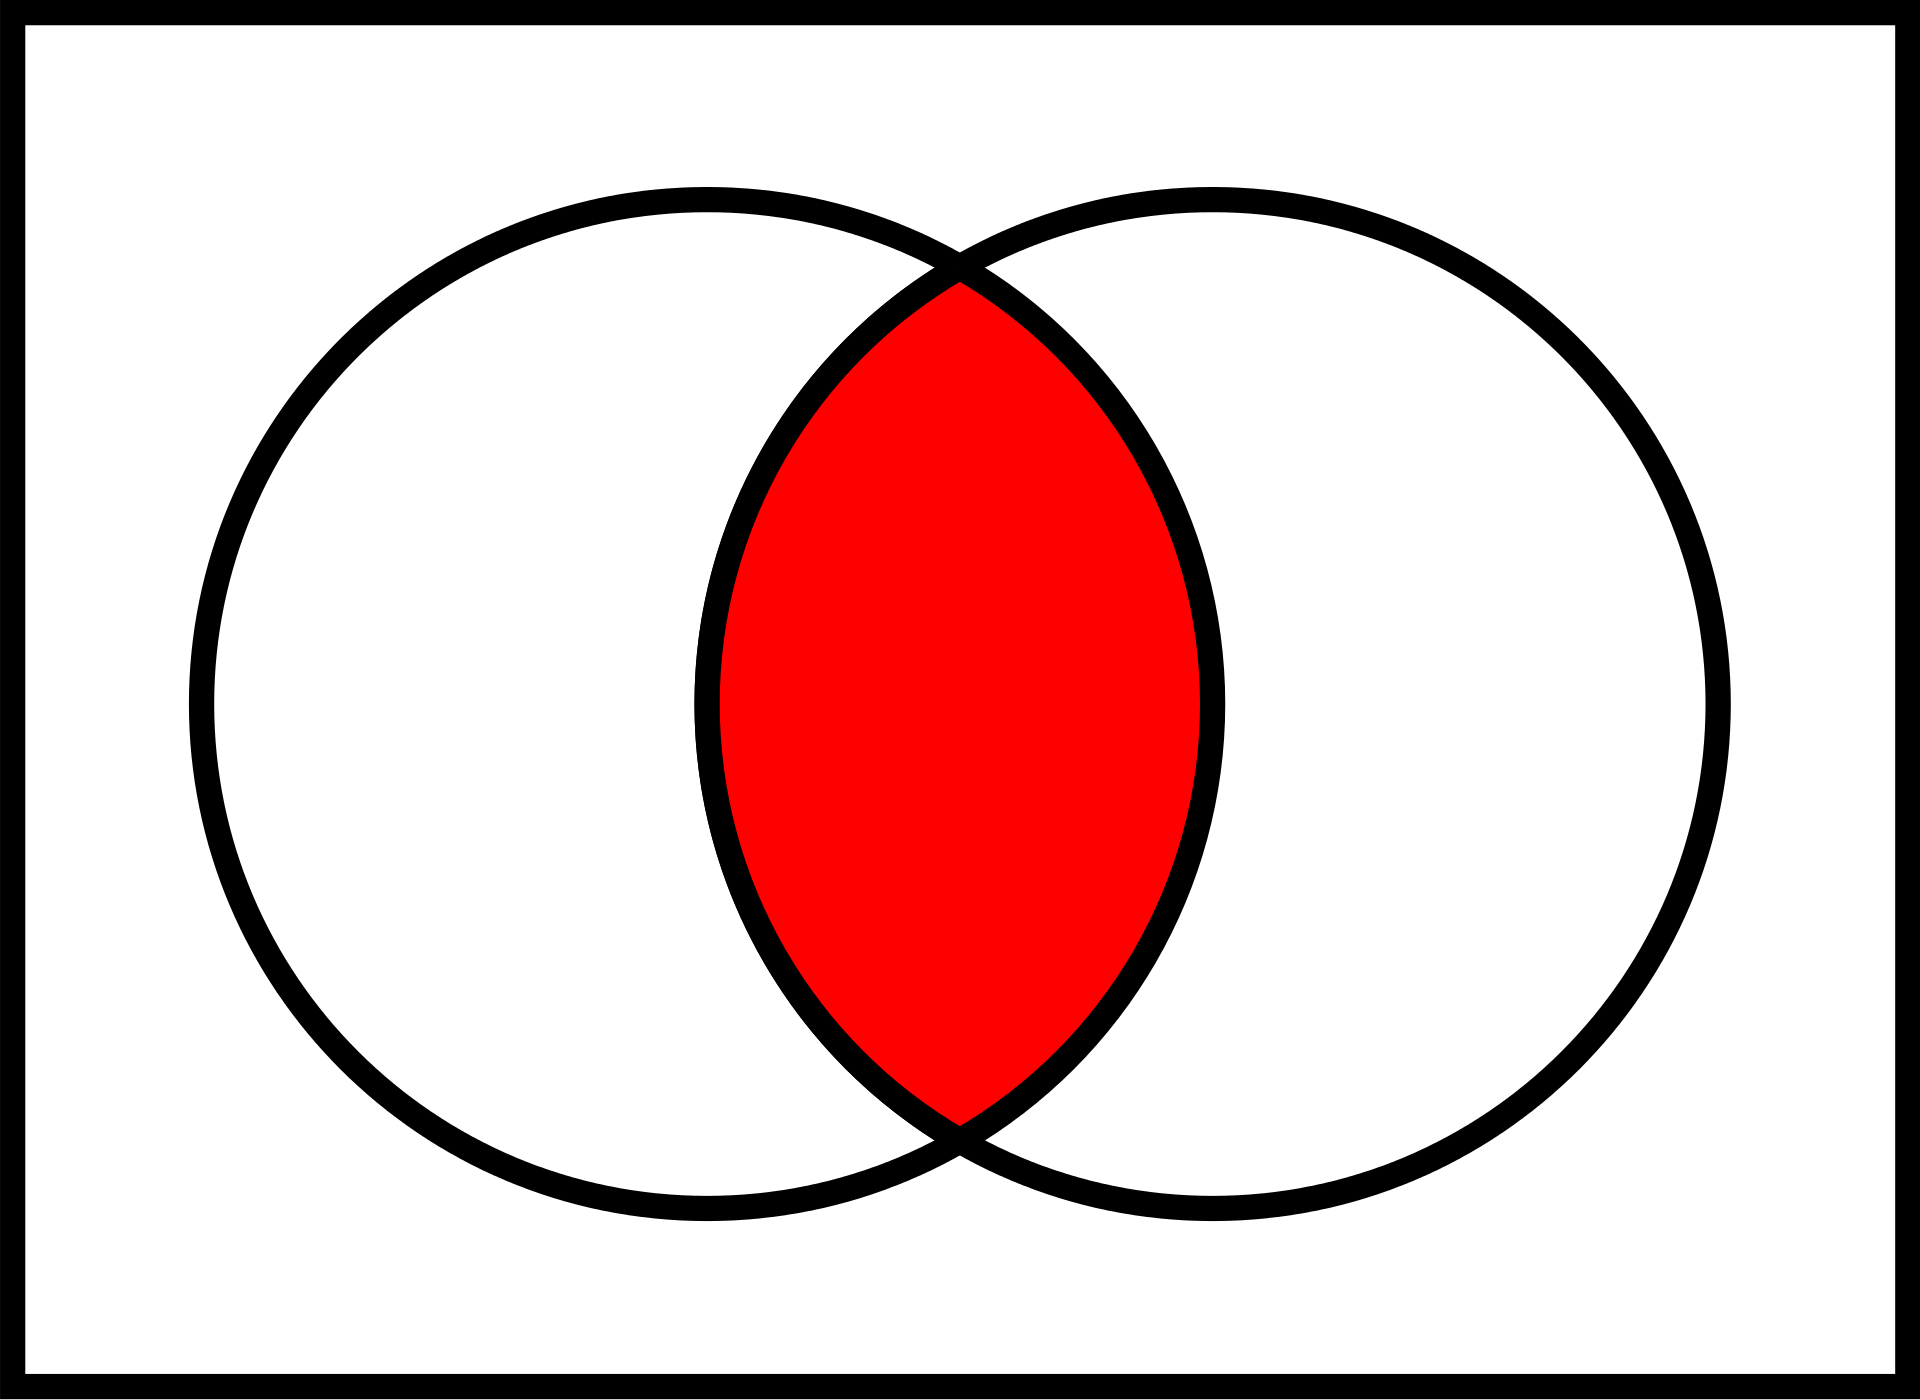
\includegraphics[width=.4\linewidth]{mehrdimWktrechnung/Venn0001.svg.png}
      \captionof*{figure}{Schnittmenge \(A\cap B\)}
      \label{fig:schnittmenge}
    \end{minipage}%
    \begin{minipage}{.5\textwidth}
      \centering
      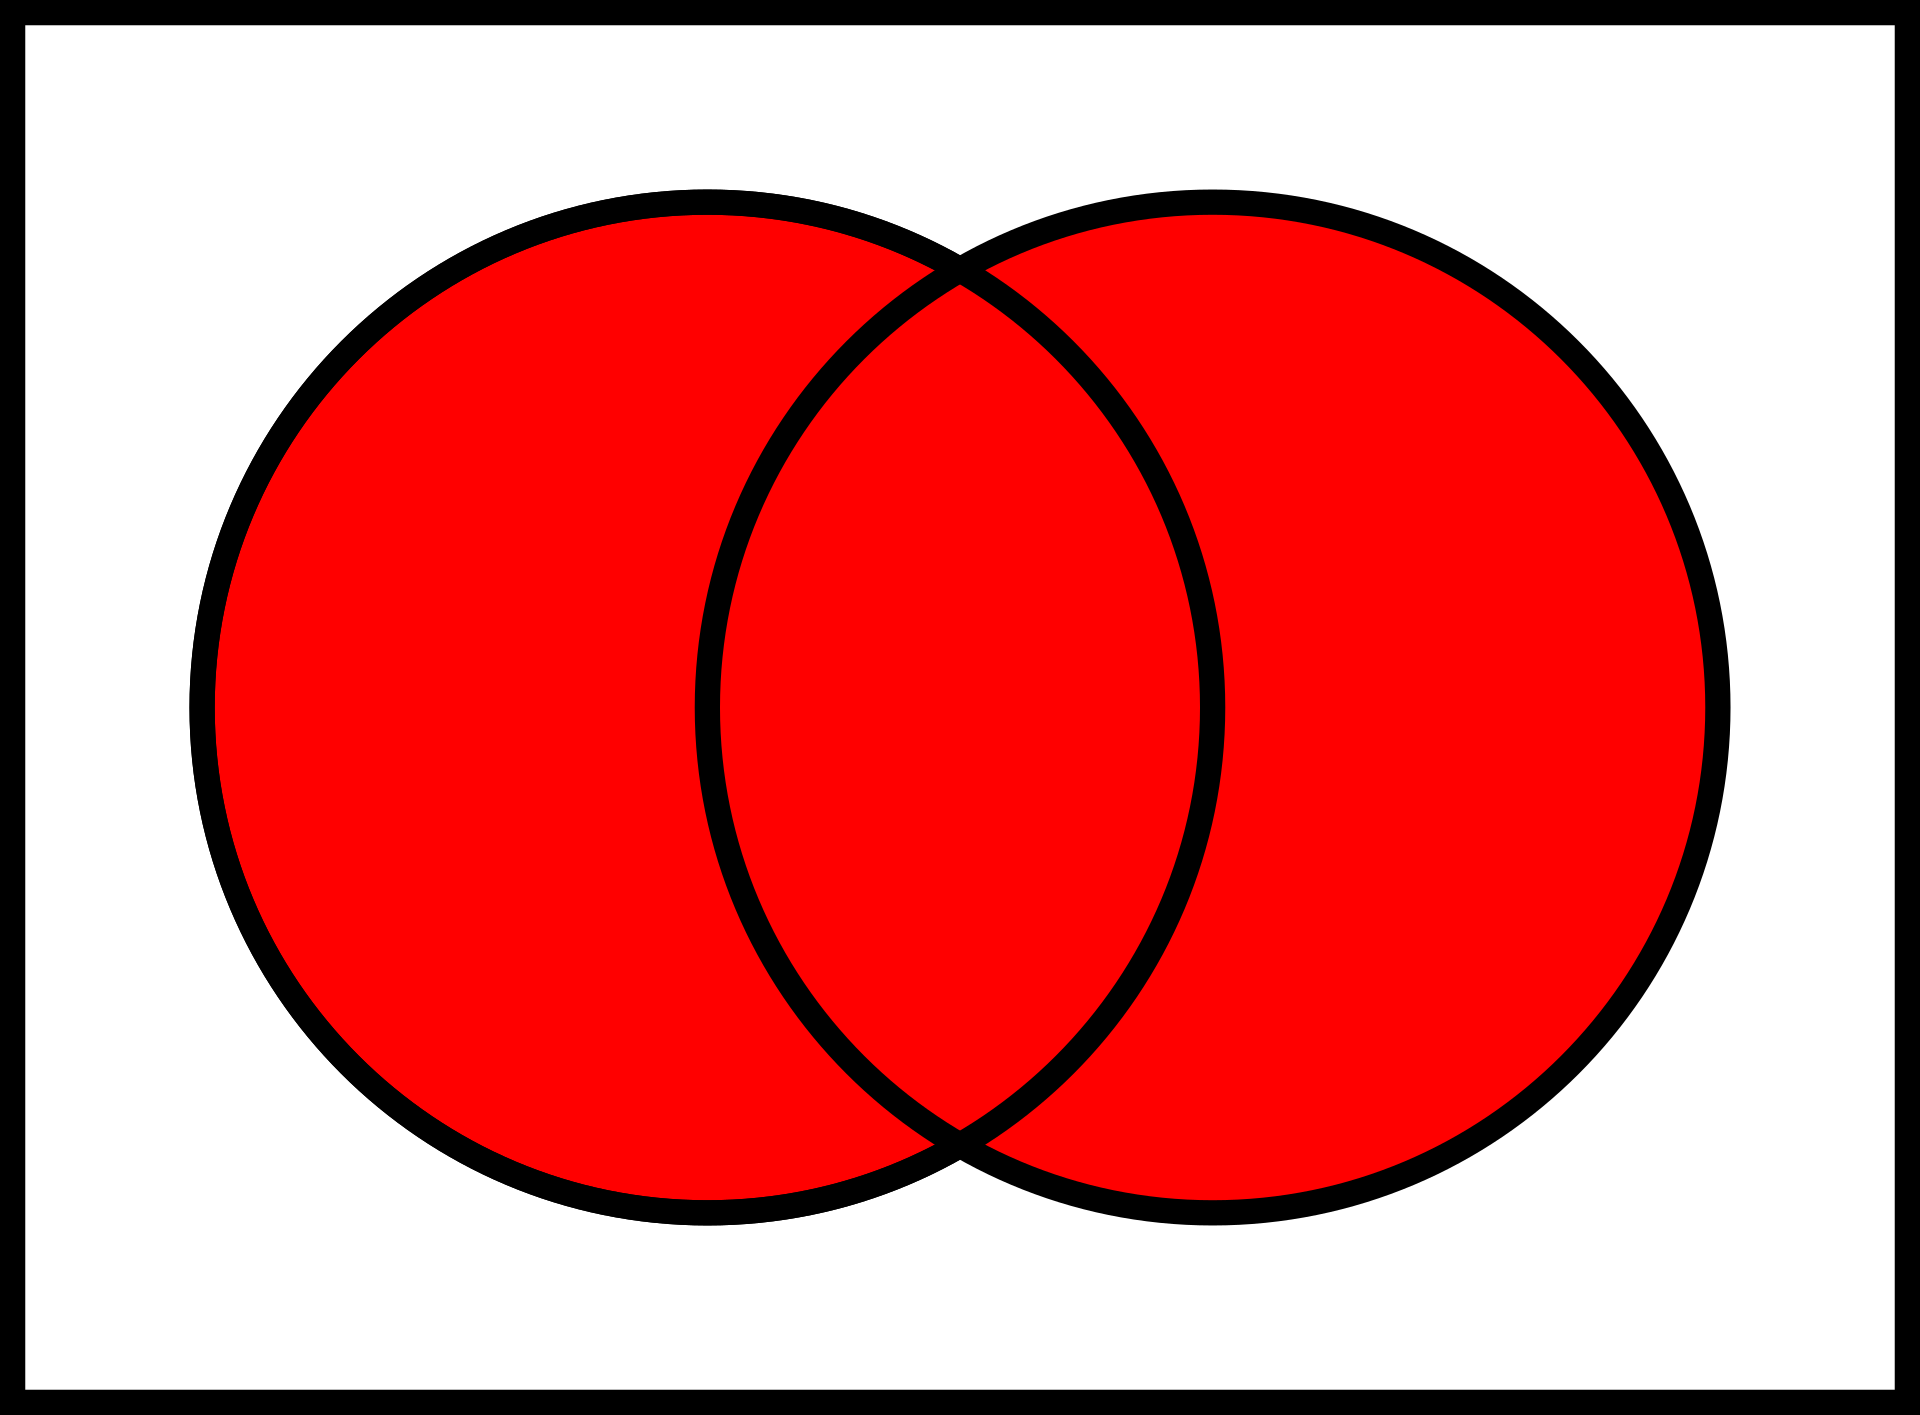
\includegraphics[width=.4\linewidth]{mehrdimWktrechnung/Venn0111.svg.png}
      \captionof*{figure}{Vereinigung \(A\cup B\)}
      \label{fig:vereinigungsmenge}
    \end{minipage}
\end{figure}

\begin{equation*}
    A\cup B = A+B-A\cap B
\end{equation*}

\subsubsection{Konvergenz}

\begin{itemize}
    \item \textbf{in Wahrscheinlichkeit}: \(X_n \xrightarrow{P} X\) wenn \(\forall \epsilon > 0: \lim_{n\rightarrow\infty}P(|X_n-EW(X)| \geq\epsilon)=\\=P(X_n \geq\epsilon)=P(X_1\geq\epsilon)\times \hdots \times P(X_n\geq\epsilon)=(1-\epsilon)^n = 0\) für \(X_n\) unab. und gleichverteilt in [0,1]
    \item \textbf{im p-ten Mittel/in \(\mathcal{L}^p\)}: \(X_n \xrightarrow{\mathcal{L}^p} X\) wenn \(\lim_{n\rightarrow\infty}E(|X_n-X|^p)\)
    \item \textbf{fast sicher}: \(X_n \xrightarrow{fs} X\) wenn \(P(\lim_{n\rightarrow\infty}X_n=X)=1\)
\end{itemize}

Konvergenz bei einer Summe von Zufallsvariablen: \(X_n \rightarrow a\) und \(Y_n \rightarrow b \Longrightarrow X_n + Y_n \rightarrow a + b\)

\subsection{Bedingte Wahrscheinlichkeit}

\begin{equation*}
    P(A|B)=\frac{P(A\cap B)}{P(B)}
\end{equation*}

\subsection{Bayes-Theorem}

\begin{equation*}
    P(A|B)=\frac{P(B|A)P(A)}{P(B)}
\end{equation*}
